\documentclass[final,hyperref={pdfpagelabels=false}]{beamer}

\mode<presentation>
  {
  %  \usetheme{Berlin}
  \usetheme{uclposter}
  \usecolortheme{ucl}

  \setbeamercolor{block body}{bg=white,fg=black}


  }
  \usepackage{times}
  \usepackage{amsmath,amsthm, amssymb, latexsym}
  \boldmath
  \usepackage[english]{babel}
  \usepackage[latin1]{inputenc}
  \usepackage[orientation=landscape,size=a0,scale=1.4,debug]{beamerposter}

  %%%%%%%%%%%%%%%%%%%%%%%%%%%%%%%%%%%%%%%%%%%%%%%%%%%%%%%%%%%%%%%%%%%%%%%%%%%%%%%%%5
  \graphicspath{{figures/}}
  \title[GVHD]{Computational analysis of gene expression datasets to unravel the basis of graft versus host disease}
  \author[Winship \& Plagnol]{Claire Winship, many others, Ron Chakraverty, Vincent Plagnol}
  \institute[UGI]{UCL Genetics Institute}
  \date{\today}



  %%%%%%%%%%%%%%%%%%%%%%%%%%%%%%%%%%%%%%%%%%%%%%%%%%%%%%%%%%%%%%%%%%%%%%%%%%%%%%%%%5
  \begin{document}

  \begin{frame}{} 

  \begin{beamercolorbox}{}
    \maketitle
  \end{beamercolorbox}


    \vfill
    \begin{columns}[t]

      \begin{column}{.25\linewidth}
        \begin{block}{Graft versus host disease}
          \begin{itemize}
          \item some items
          \item some items
          \item some items
          \item some items
          \end{itemize}
        \end{block}


        \begin{block}{The ImmGene project}
          \begin{itemize}
          \item some items
          \item some items
          \item some items
          \item some items
          \end{itemize}
        \end{block}

      \end{column}


      \begin{column}{.24\linewidth}
        \begin{block}{T-cell expression in multiple minor histocompatibility antigen-mismatched BMT model}
	  {\bf Objective:} In a polyclonal model, evaluate the differences in gene expression of effector T cells found in the lymphoid organs or in the peripheral tissues.

	  \begin{minipage}{0.45\textwidth}
	    \includegraphics[width=13cm]{/cluster/project8/vyp/Winship_GVHD/claire/results/mhc1_ko/figs/PCA_prettier.pdf}
	  \end{minipage}	  
	  \begin{minipage}{0.45\textwidth}
	    \includegraphics[width=13cm]{/cluster/project8/vyp/Winship_GVHD/claire/results/mhc1_ko/figs/PCA_prettier_outlier_removed.pdf}
	  \end{minipage}	  
	  
          \begin{itemize}
          \item PCA analysis of all samples reveals presence of outlier in the D7 dataset ($TM008_ko4$)
          \item some items
          \item some items
          \end{itemize}
	  \begin{minipage}{0.45\textwidth}
            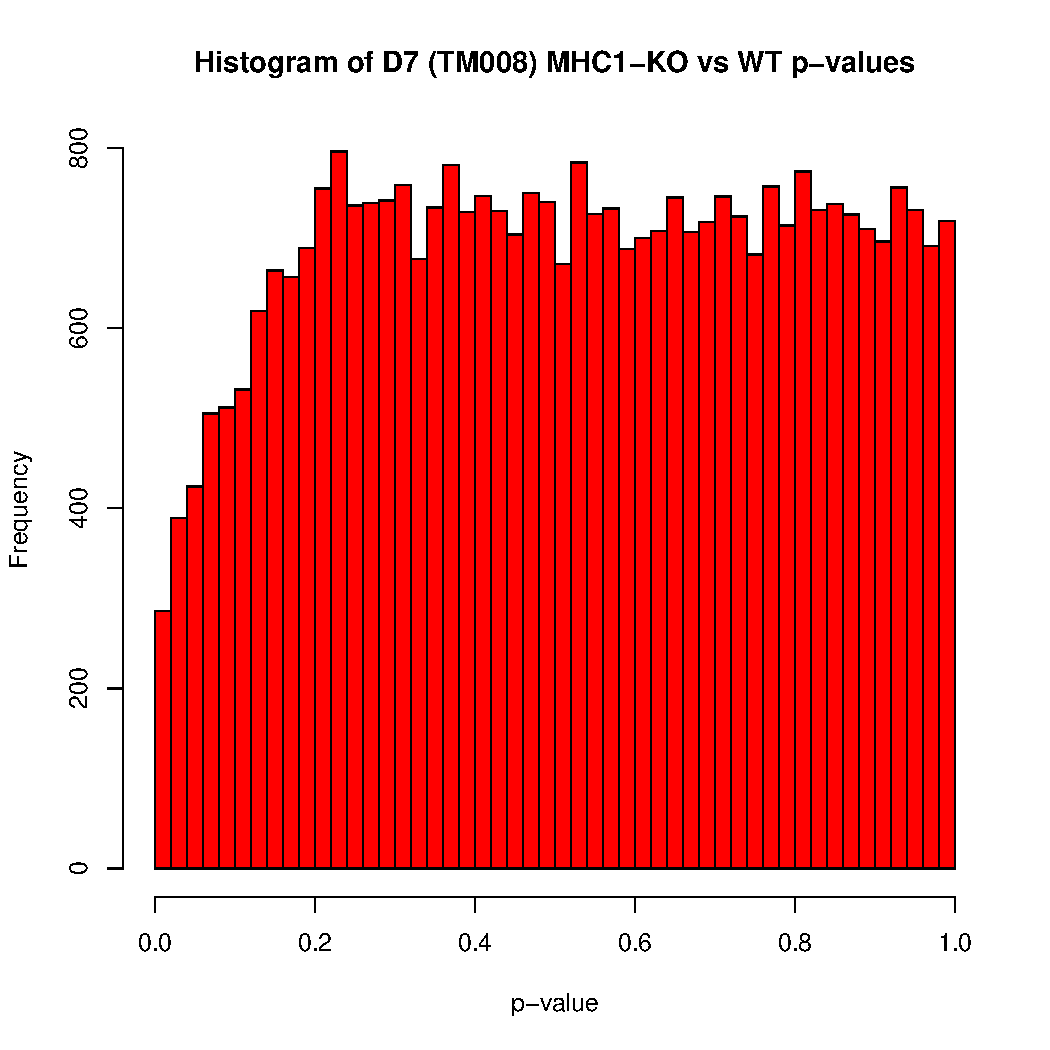
\includegraphics[width=13cm]{/cluster/project8/vyp/Winship_GVHD/claire/results/mhc1_ko/figs/D7_histogram.pdf}
          \end{minipage}
	  \begin{minipage}{0.45\textwidth}
            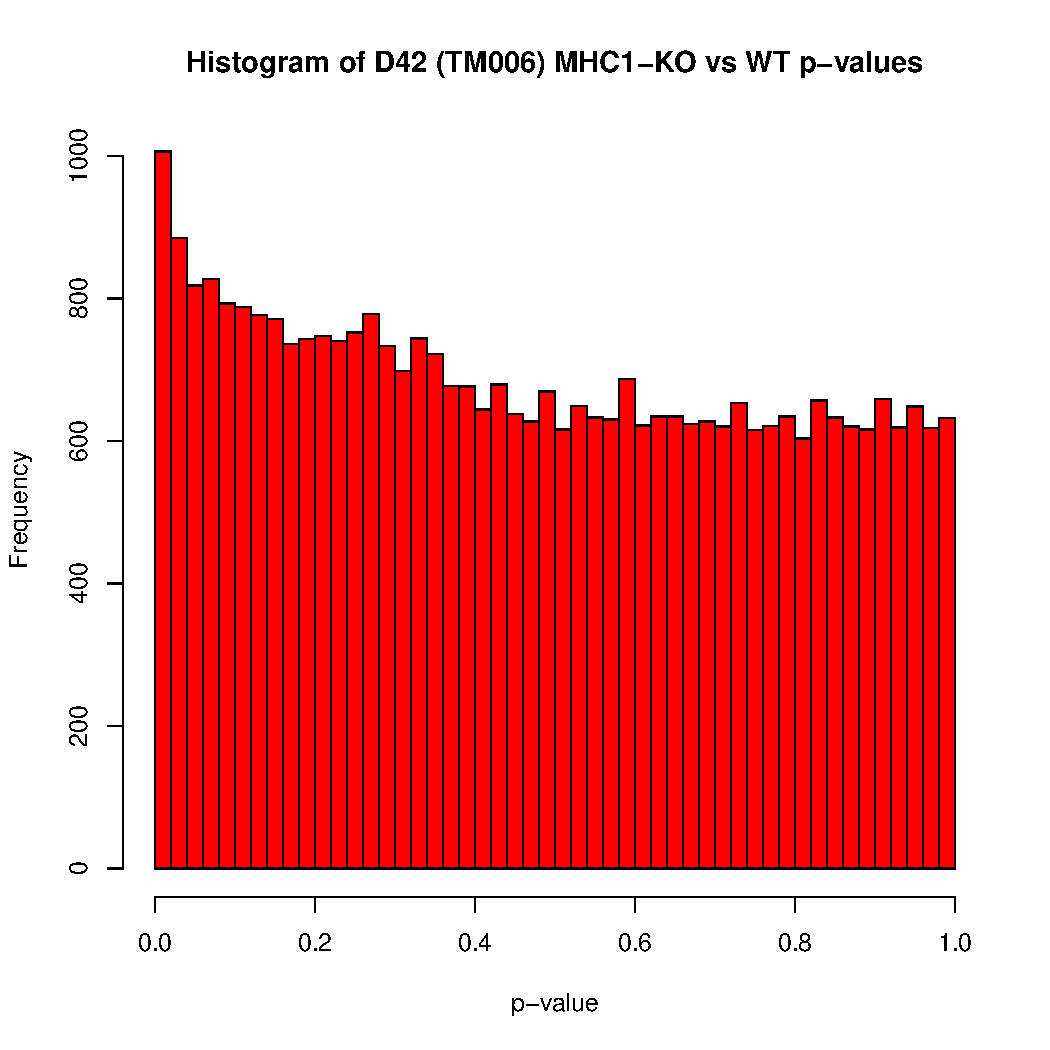
\includegraphics[width=13cm]{/cluster/project8/vyp/Winship_GVHD/claire/results/mhc1_ko/figs/D42_histogram.pdf}
          \end{minipage}
	  \begin{itemize}
	    \item some items
	    \item some items
	    \end{itemize}
          \begin{minipage}{0.45\textwidth}
            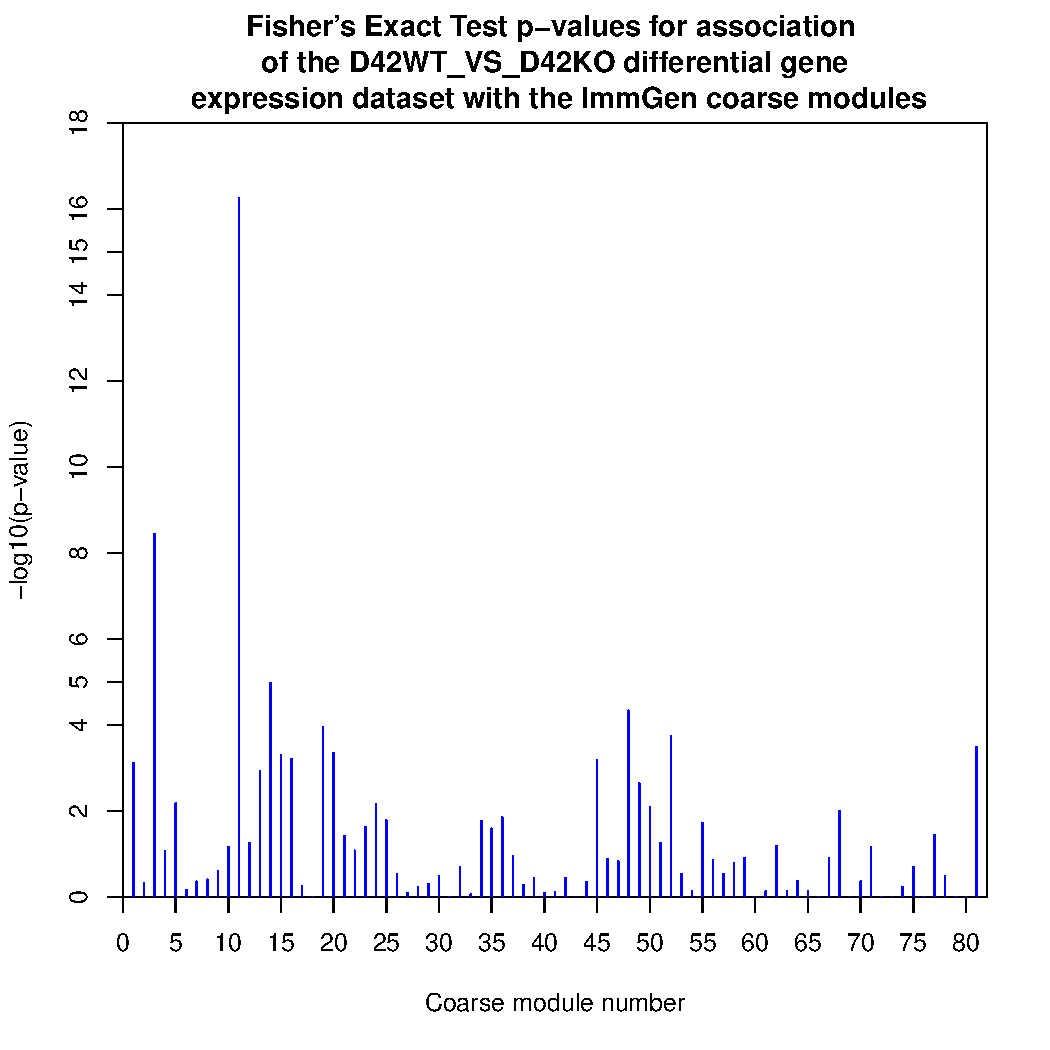
\includegraphics[width=13cm]{/cluster/project8/vyp/Winship_GVHD/claire/results/mhc1_ko/figs/D42WT_VS_D42KO_coarse_module_association_graph.pdf}
          \end{minipage}
          \begin{minipage}{0.45\textwidth}
            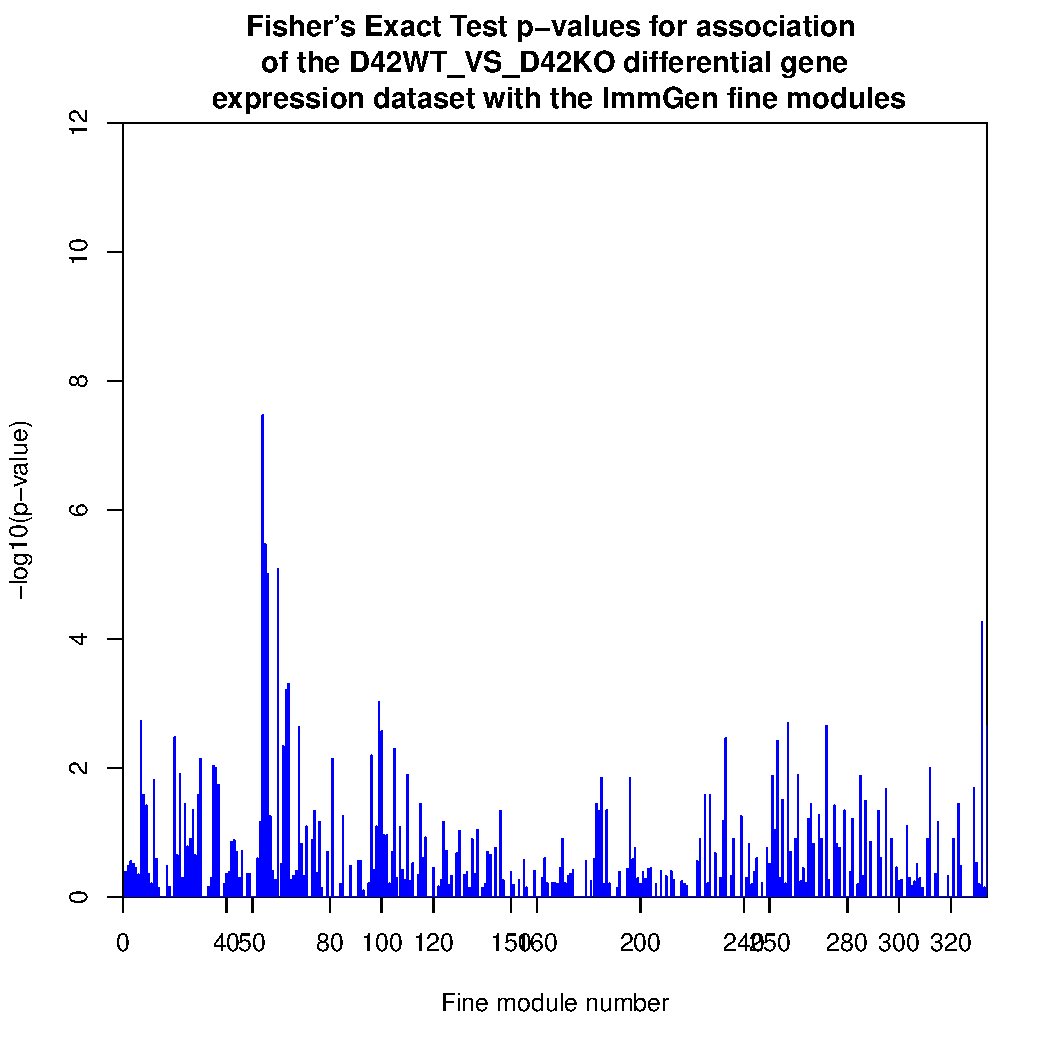
\includegraphics[width=13cm]{/cluster/project8/vyp/Winship_GVHD/claire/results/mhc1_ko/figs/D42WT_VS_D42KO_fine_module_association_graph.pdf}
          \end{minipage}
	  \begin{center}
	    \begin{tabular}{ |c|c|c| } 
	      \hline
	      gene name & fold change & pvalue \\
	      \hline
	      Ptbp2 & 0.8575669378 & 0.0002380649 \\
	      Trappc1 & -0.8105321657 & 0.0011522667 \\
	      Mrpl32 & -0.9482075354 & 0.0015174569 \\
	      Ctso & 0.6665616898 & 0.0015502065 \\
	      Cib1 & -0.5435813927 & 0.0022304297 \\
	      Chordc1  & -1.1641319443 & 0.0033252187 \\
	      Actr6 & -0.7619741241 & 0.0034636625 \\
	      Pcgf5 & -0.6144202783 & 0.0035618031 \\
	      Llph & -0.797961394 & 0.0047160713 \\
	      1810037I17Rik & -0.6327137658 & 0.0053622021 \\
	      Cd46 & 1.2478436705 & 0.0077584292 \\
	      Zfp455 & -1.3221395229 & 0.0083646381 \\
	      \hline
	    \end{tabular}
	  \end{center}
        \end{block}
      \end{column}
      \begin{column}{.25\linewidth}
        \begin{block}{T-cell expression: Single minor histocompatibility antigen-mismatched BMT model}
	  {\bf Objective:} In a monoclonal model, evaluate the effect of depleting Langerhans cells on the gene expression of effector T cells found in the lymph nodes and in the skin.
	  \begin{center}
	   \includegraphics[width=15cm]{/cluster/project8/vyp/Winship_GVHD/claire/results/epi_dermis_PLN/figs/PCA_prettier.pdf}
            \end{center}
          \begin{itemize}
          \item some items
          \item some items
          \item some items
          \item some items
          \end{itemize}
	  \begin{minipage}{0.45\textwidth}
            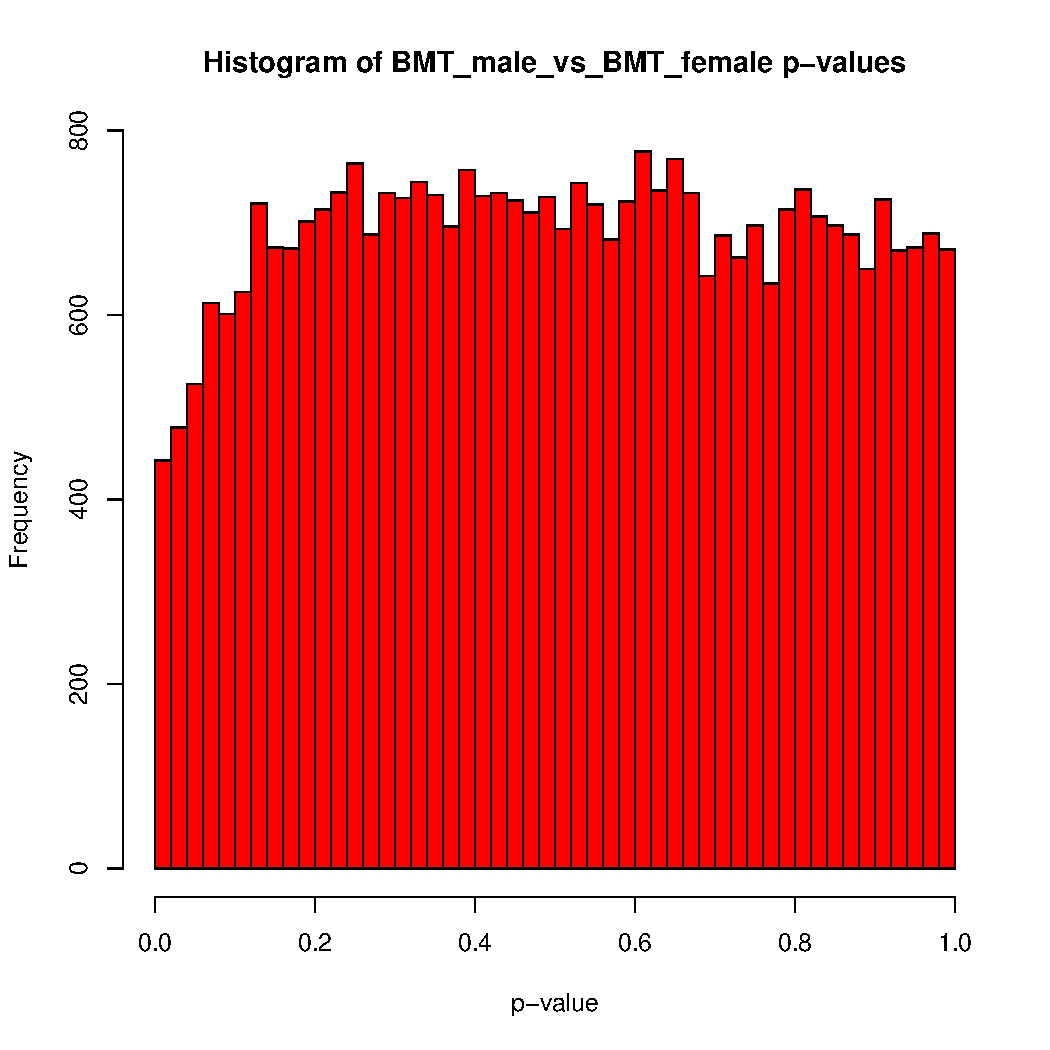
\includegraphics[width=13cm]{/cluster/project8/vyp/Winship_GVHD/claire/results/syn_allo_bmt/figs/BMT_male_vs_BMT_female_histogram.pdf}
          \end{minipage}
          \begin{minipage}{0.45\textwidth}
            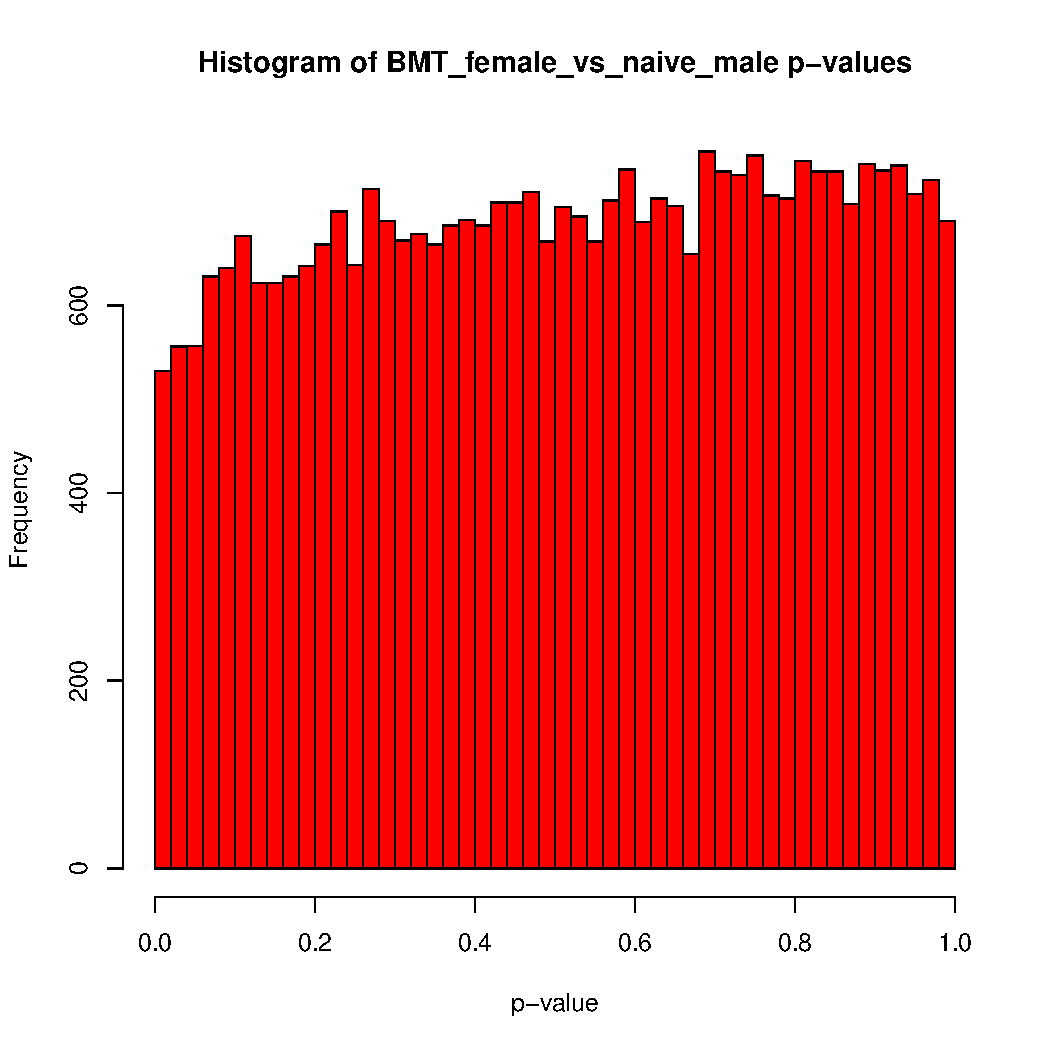
\includegraphics[width=13cm]{/cluster/project8/vyp/Winship_GVHD/claire/results/syn_allo_bmt/figs/BMT_female_vs_naive_male_histogram.pdf}
          \end{minipage}
	  \begin{minipage}{0.45\textwidth}
            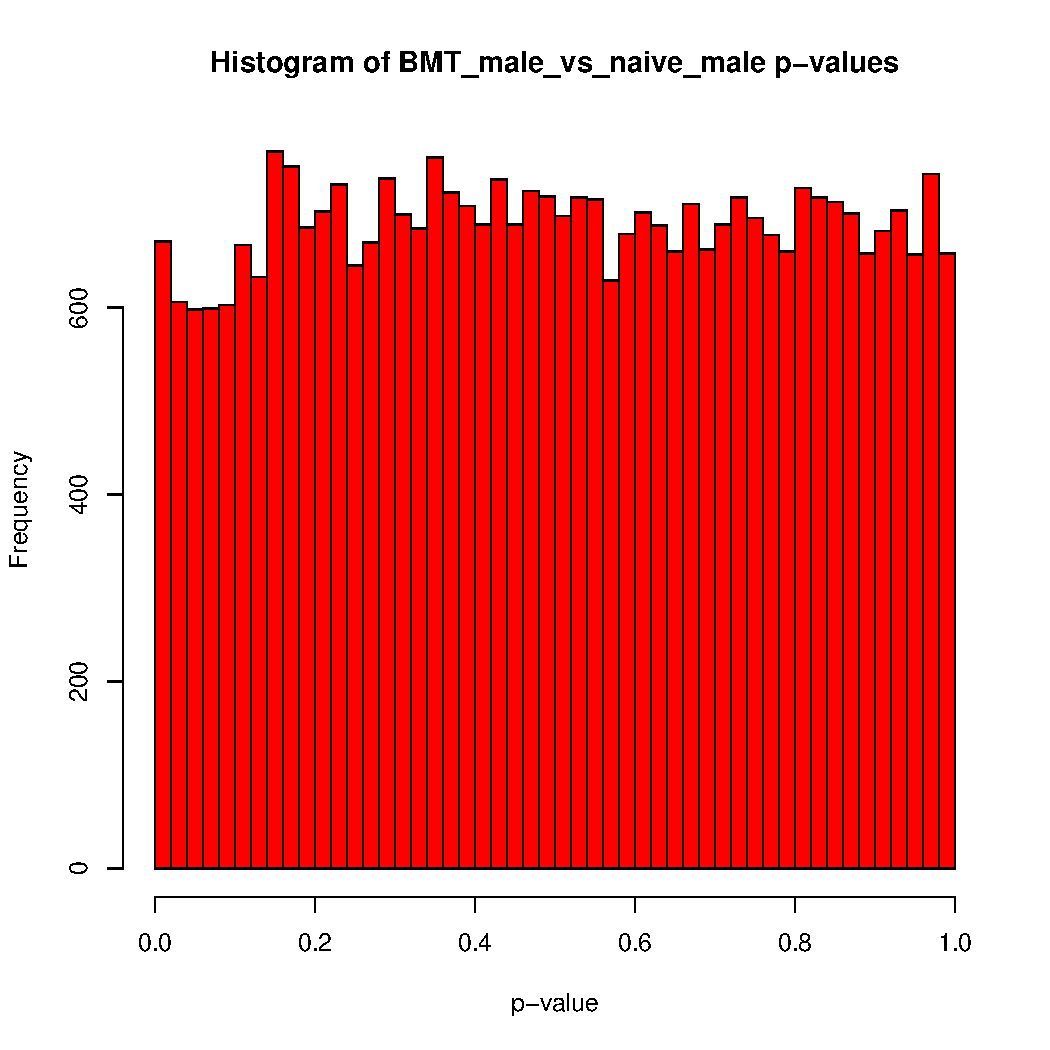
\includegraphics[width=13cm]{/cluster/project8/vyp/Winship_GVHD/claire/results/syn_allo_bmt/figs/BMT_male_vs_naive_male_histogram.pdf}
          \end{minipage}
	  \begin{itemize}
	    \item some items
	    \item some items
	   \end{itemize}
	  \begin{minipage}{0.45\textwidth}
            \includegraphics[width=13cm]{/cluster/project8/vyp/Winship_GVHD/claire/results/syn_allo_bmt/figs/BMT_male_vs_BMT_female_coarse_module_association_graph.pdf}
          \end{minipage}

	   \begin{minipage}{0.45\textwidth}
            \includegraphics[width=13cm]{/cluster/project8/vyp/Winship_GVHD/claire/results/syn_allo_bmt/figs/BMT_male_vs_BMT_female_fine_module_association_graph.pdf}
          \end{minipage}
          \begin{minipage}{0.45\textwidth}
            \includegraphics[width=13cm]{/cluster/project8/vyp/Winship_GVHD/claire/results/syn_allo_bmt/figs/BMT_female_vs_naive_male_coarse_module_association_graph.pdf}
          \end{minipage}
	  \begin{minipage}{0.45\textwidth}
            \includegraphics[width=13cm]{/cluster/project8/vyp/Winship_GVHD/claire/results/syn_allo_bmt/figs/BMT_female_vs_naive_male_fine_module_association_graph.pdf}
          \end{minipage}
          \begin{minipage}{0.45\textwidth}
            \includegraphics[width=13cm]{/cluster/project8/vyp/Winship_GVHD/claire/results/syn_allo_bmt/figs/BMT_male_vs_naive_male_coarse_module_association_graph.pdf}
          \end{minipage}
	  \begin{minipage}{0.45\textwidth}
            \includegraphics[width=13cm]{/cluster/project8/vyp/Winship_GVHD/claire/results/syn_allo_bmt/figs/BMT_male_vs_naive_male_fine_module_association_graph.pdf}
          \end{minipage}
        \end{block}
      \end{column}


      \begin{column}{.25\linewidth}
        \begin{block}{Langerhans cell expression}
	  {\bf Objective:} Evaluate the differences in gene expression of Langerhans cells in the setting of an allogeneic BMT or a syngeneic BMT.
           \begin{center}
           \includegraphics[width=15cm]{/cluster/project8/vyp/Winship_GVHD/claire/results/syn_allo_bmt/figs/PCA_prettier.pdf}
          \end{center}

          \begin{itemize}
          \item some items
          \item some items
          \item some items
          \item some items
          \end{itemize}
        \end{block}
      \end{column}


    \end{columns}
  \end{frame}
\end{document}


%%%%%%%%%%%%%%%%%%%%%%%%%%%%%%%%%%%%%%%%%%%%%%%%%%%%%%%%%%%%%%%%%%%%%%%%%%%%%%%%%%%%%%%%%%%%%%%%%%%%
%%% Local Variables: 
%%% mode: latex
%%% TeX-PDF-mode: t
%%% End:
